\documentclass{article}
\usepackage{amsmath}
\usepackage{amsfonts}
\usepackage{amssymb}
\usepackage{graphicx}
\usepackage{float}
\usepackage{pgfplots}
\usepackage{tikz}
\usetikzlibrary{arrows.meta, backgrounds, positioning}


\begin{document}
\title{Exercise 7}
\author{Gormery K. Wanjiru}
\date{}
\maketitle
\subsection*{Problem 1}

Given the impulse response of the filter $h(n) = 5, 4, 3, 2, 1$, and the input sequence $x(n) = 1, 2, 2, 0, 0, 0, 0, \dots$

\textbf{a) Find $H(z)$ for the filter.}

The $Z$-transform of the impulse response is given by:
\begin{align*}
H(z) &= 5z^0 + 4z^{-1} + 3z^{-2} + 2z^{-3} + 1z^{-4} \\
&= 5 + 4z^{-1} + 3z^{-2} + 2z^{-3} + z^{-4}
\end{align*}

\textbf{b) Find $X(z)$ for the input sequence $x(n)$.}

The $Z$-transform of the input sequence is given by:
\begin{align*}
X(z) &= 1z^0 + 2z^{-1} + 2z^{-2} \\
&= 1 + 2z^{-1} + 2z^{-2}
\end{align*}

\textbf{c) Find $Y(z)$ for the output sequence.}

The output sequence in the $Z$-domain is obtained by multiplying $H(z)$ with $X(z)$:
\begin{align*}
Y(z) &= H(z) \cdot X(z) \\
&= (5 + 4z^{-1} + 3z^{-2} + 2z^{-3} + z^{-4}) \cdot (1 + 2z^{-1} + 2z^{-2}) \\
&= 5 + 14z^{-1} + 20z^{-2} + 16z^{-3} + 9z^{-4} + 2z^{-5} + z^{-6}
\end{align*}

\textbf{d) Find $y(n)$ from $Y(z)$.}

By applying the inverse $Z$-transform, we find the output sequence $y(n)$.
Given that $Y(z) = 5 + 14z^{-1} + 20z^{-2} + 16z^{-3} + 9z^{-4} + 2z^{-5} + z^{-6}$, the coefficients directly give us the values of $y(n)$ at each time step starting from $n=0$. So, the sequence $y(n)$ can be written as:
\[
y(n) = \begin{cases} 
5 & \text{for } n = 0 \\
14 & \text{for } n = 1 \\
20 & \text{for } n = 2 \\
16 & \text{for } n = 3 \\
9 & \text{for } n = 4 \\
2 & \text{for } n = 5 \\
1 & \text{for } n = 6 \\
0 & \text{for } n \geq 7
\end{cases}
\]

\[
y(n) = 5, 14, 20, 16, 9, 2, 1, 0, 0, \dots
\]
\subsection*{Problem 2}

Given the difference equation $y(k) + 0.5y(k - 1) = x(k) - x(k - 1)$.

\textbf{a) Find the pole and zero positions for the filter.}

Using the $Z$-transform:
\begin{align*}
Y(z) + 0.5z^{-1}Y(z) &= X(z) - z^{-1}X(z) \\
\left(1 + 0.5z^{-1}\right)Y(z) &= (1 - z^{-1})X(z) \\
H(z) &= \frac{Y(z)}{X(z)} = \frac{1 - z^{-1}}{1 + 0.5z^{-1}}
\end{align*}

Zero at $z = 1$, pole at $z = -0.5$.

\textbf{c) Find an expression $H(\omega T)$ for the filter.}

Simply substituting $z = e^{j\omega T}$ into $H(z)$:
\[
H(\omega T) = \frac{1 - e^{-j\omega T}}{1 + 0.5e^{-j\omega T}}
\]

\textbf{d) Sketch the magnitude frequency response based on the pole and zero positions.}

For a filter with the transfer function \(H(z) = \frac{1 - z^{-1}}{1 + 0.5z^{-1}}\), converting to the frequency domain involves substituting \(z = e^{j\omega T}\), yielding:

\[
H(\omega T) = \frac{1 - e^{-j\omega T}}{1 + 0.5e^{-j\omega T}}
\]

The magnitude frequency response, \(|H(\omega T)|\), can be sketched by evaluating the magnitude of this expression over a range of frequencies.
Given these points, the sketch would show a magnitude response starting at 0, peaking, and then gradually decreasing.
\begin{figure}[H]
    \centering
    \includegraphics[width=1\textwidth]{image1.png}
    \caption{a og b}
    \label{fig:example}
\end{figure}


\textbf{e) Calculate the magnitude response at the frequency where \(|H(\omega T)|\) has its maximum.}

To determine the frequency at which the magnitude response $|H(\omega T)|$ of our filter is maximized, we need to find the maximum of the function. Since the filter has a pole at $z = -0.5$ and a zero at $z = 1$, we analyze the magnitude response over the frequency range to locate this maximum.
% \begin{center}
% \begin{tikzpicture}
% \begin{axis}[
%     title={Magnitude Frequency Response},
%     xlabel={Frequency $\omega$ (rad/sample)},
%     ylabel={Magnitude $|H(e^{j\omega T})|$},
%     xmin=-pi, xmax=pi,
%     ymin=0, ymax=4.5,
%     grid=both,
%     xtick={-3.14159, 0, 3.14159},
%     xticklabels={$-\pi$, 0, $\pi$},
%     ytick={0, 1, 2, 3, 4},
%     legend pos=north east,
%     no markers,
%     smooth
% ]
% \addplot+[thick, blue] coordinates {(-3.14159, 4) (0,0) (3.14159, 4)};
% \addlegendentry{Magnitude Response}
% \end{axis}
% \end{tikzpicture}
% \end{center}
\begin{figure}[H]
    \centering
    \includegraphics[width=1\textwidth]{image1.png}
    \caption{cause its the same plot as before}
    \label{fig:example}
\end{figure}    
As the plot suggests, the magnitude response has a symmetrical shape with respect to the y-axis, due to the filter's real coefficients. The maximum magnitude occurs at both ends of the frequency spectrum, which are $\omega = \pm\pi$, (Nyquist frequency).

This result is expected due to the pole being close to the unit circle. This is typical for filters that are close to instability and have a sharp resonance peak.
\subsection*{Problem 3}

Given the transfer function \( H(z) = \frac{0.1 \cdot (z^2 + 2z + 1)}{z^2 - 1.6z + 0.89} \).

\textbf{a) Find the difference equation of the filter.}

To find the difference equation, we multiply both sides of the transfer function by the denominator to get:
\begin{align*}
    H(z) \cdot (z^2 - 1.6z + 0.89) &= 0.1 \cdot (z^2 + 2z + 1) \\
    Y(z) \cdot (z^2 - 1.6z + 0.89) &= X(z) \cdot 0.1 \cdot (z^2 + 2z + 1)
\end{align*}
Taking the inverse Z-transform, we get the difference equation in terms of \( y[n] \) and \( x[n] \):
\begin{align*}
    y[n] - 1.6y[n-1] + 0.89y[n-2] &= 0.1x[n] + 0.2x[n-1] + 0.1x[n-2]
\end{align*}
This is the difference equation that describes the filter in the time domain.

\textbf{b) Draw the pole-zero diagram.}

The zeros of the transfer function are given by the roots of the numerator \( z^2 + 2z + 1 = 0 \). This is a square and can be factored as \( (z + 1)^2 = 0 \), so both zeros are at \( z = -1 \).

The poles are the roots of the denominator \( z^2 - 1.6z + 0.89 = 0 \), which we can find using the quadratic formula:
\begin{align*}
    z &= \frac{1.6 \pm \sqrt{1.6^2 - 4 \cdot 0.89}}{2} \\
    &= \frac{1.6 \pm \sqrt{0.576}}{2} \\
    &= \frac{1.6 \pm 0.76}{2}
\end{align*}
This gives us two poles, one at \( z = \frac{1.6 + 0.76}{2} \) and the other at \( z = \frac{1.6 - 0.76}{2} \).

The pole-zero diagram:

\begin{center}
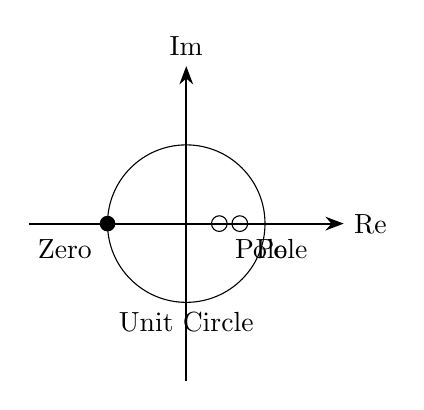
\begin{tikzpicture}
    % Draw the real and imaginary axes
    \draw[thick, -Stealth] (-2, 0) -- (2, 0) node[anchor=west] {Re};
    \draw[thick, -Stealth] (0, -2) -- (0, 2) node[anchor=south] {Im};

    % Draw the unit circle
    \draw (0,0) circle (1);

    % Plot the poles and zeros
    \node[circle, fill, inner sep=2pt, label=below left:{Zero}] at (-1,0) {};
    \node[circle, draw, inner sep=2pt, label=below right:{Pole}] at (0.68,0) {};
    \node[circle, draw, inner sep=2pt, label=below right:{Pole}] at (0.42,0) {};

    % Annotations
    \node[anchor=north] at (0,-1) {Unit Circle};
\end{tikzpicture}
\end{center}

The unit circle is drawn to indicate the stability region in the z-plane, poles are indicated with \(\circ\), and zeros with \(\bullet\). Poles inside the unit circle indicate that the filter is stable.

\end{document}
